% Created 2019-09-03 di 11:17
% Intended LaTeX compiler: pdflatex
\documentclass[final]{beamer}
	         \usetheme{ph}
           \usepackage[orientation=portrait,size=a0,scale=1.4]{beamerposter}
           \usepackage[absolute,overlay]{textpos}
	         \usepackage[authoryear]{natbib}


\setlength{\paperwidth}{36in}
\setlength{\paperheight}{48in}
\setlength{\textwidth}{0.98\paperwidth}
\setlength{\textheight}{0.98\paperheight}
\graphicspath{{../output/figures/}{../lib/}}
\usepackage[export]{adjustbox}
\usepackage{graphicx,caption}
\usepackage{minted}
\usepackage{eurosym}
\usepackage{listings}
\usepackage{textcomp}
\usepackage{bibentry}
\newcommand\sumin{\sum_{i=1}^{n}}
\newcommand{\Xoi}[1]{#1(i)}
\newcommand{\frakPQ}[2]{\frac{\Xoi{#1}}{\Xoi{#2}}}
\newcommand{\DKLPQ}[3]{D_{\mathrm{KL}}(#1 #3 #2)}
\date{}
\newcommand{\auth}{Iris Yuping Ren}
\newcommand{\authemail}{y.ren@uu.nl}
\newcommand{\authtwitter}{@irisyupingren}
\newcommand{\authgithub}{github.com/irisyupingren}
\author{
Orestis Melkonian$^{1}$, Iris Yuping Ren$^{1}$, Wouter Swierstra$^{1}$, Anja Volk$^{1}$
\\
\vspace{5mm}
\normalsize{$^{1}$Department of Information and Computing Sciences,}
\normalsize{Utrecht University}
}
\usetheme{default}
\date{2019-09-03 11:17}
\title{What constitutes a musical pattern?}
\begin{document}

\begin{frame}[label={sec:orgd59d0ad},fragile]{}
 \vspace{-2cm}
\begin{columns}
\begin{column}[t]{0.47\columnwidth}
\begin{block}{Background}
\begin{itemize}
\item Musical patterns are diverse.
\item Evaluation of pattern discovery algorithms is hard.
\end{itemize}

\begin{columns}
\begin{column}[T]{0.90\columnwidth}
\begin{figure}[htbp]
\centering
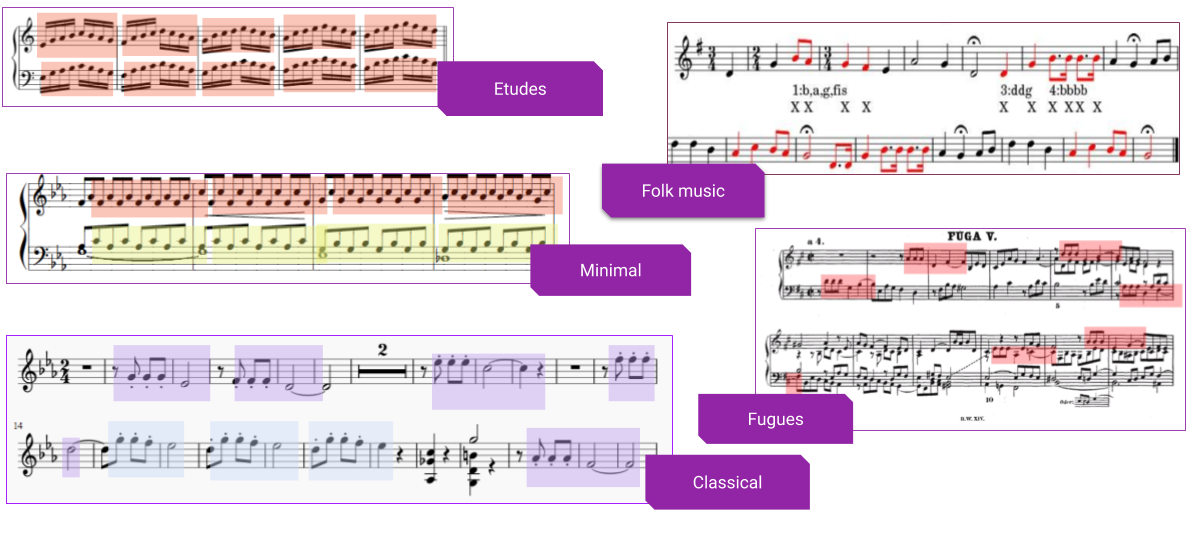
\includegraphics[width=.9\linewidth]{img/examples.png}
\caption{\label{fig:orgd0df8ba}
Patterns in music}
\end{figure}


\begin{figure}[htbp]
\centering
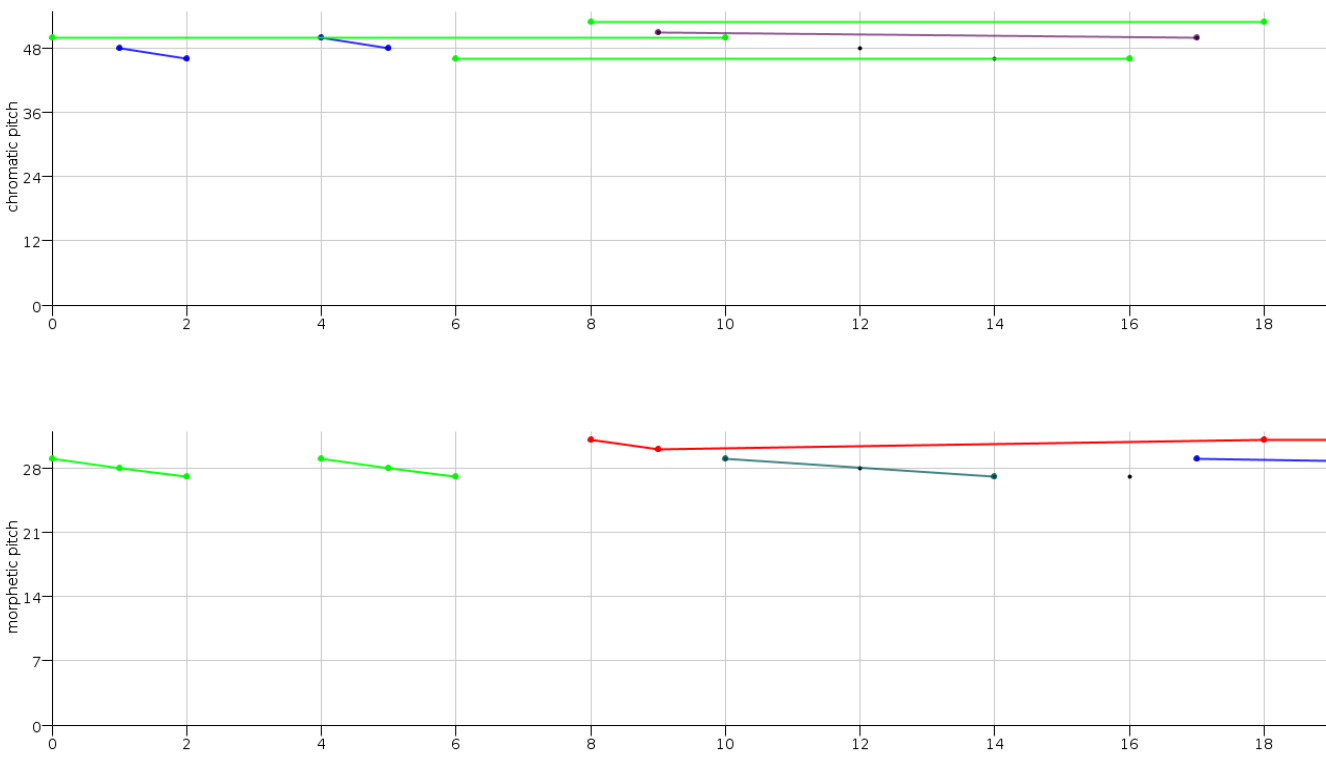
\includegraphics[width=.9\linewidth]{img/alg.png}
\caption{\label{fig:orgf369048}
Same music, different algorithms discover different patterns}
\end{figure}
\end{column}
\end{columns}
\end{block}
\begin{block}{Musical Transformations}
Taking a relative perspective, relate occurrences to each other via musical transformations: 
\(Occurrence 1 <=> Occurrence 2\)

\begin{columns}
\begin{column}[T]{0.85\columnwidth}
\begin{center}
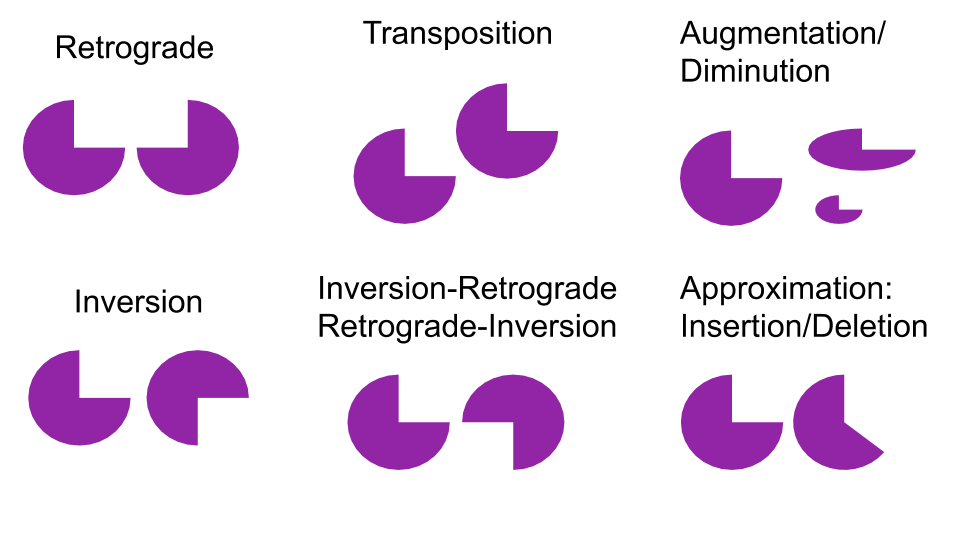
\includegraphics[width=.9\linewidth]{img/transformations.png}
\end{center}
\end{column}
\end{columns}
\end{block}


\begin{block}{Assembling checkers: Contravariant Bifunctor}
\begin{columns}
\begin{column}[T]{0.85\columnwidth}
\begin{minted}[linenos=false,bgcolor=white,breaklines=true]{haskell}
checkBasedOnTime :: (Pattern -> Time) -> HomCheck Time -> HomCheck Pattern
\end{minted}

\begin{center}
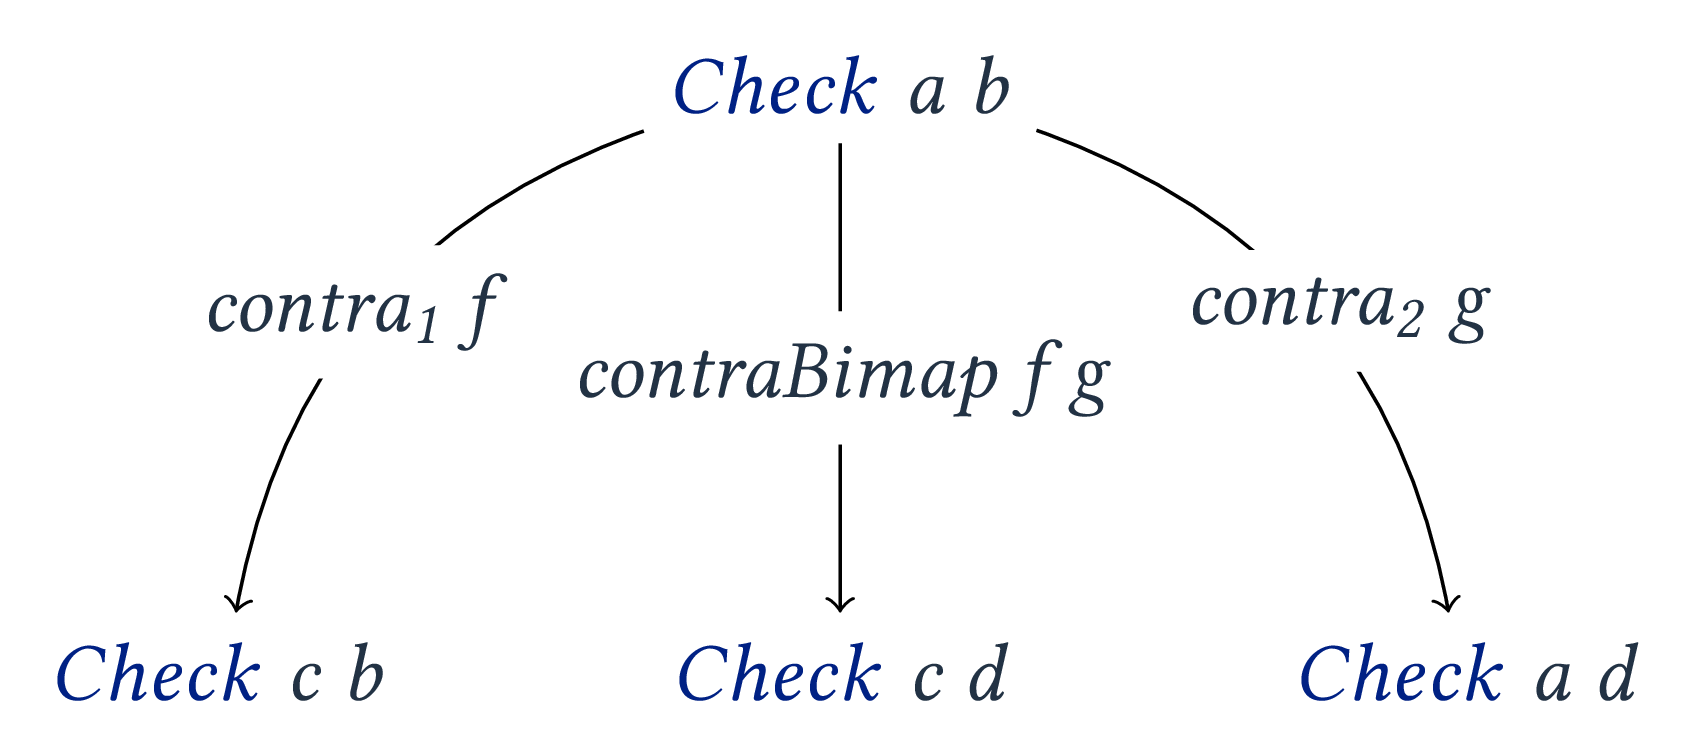
\includegraphics[width=.9\linewidth]{./img/contra.png}
\end{center}
\end{column}
\end{columns}
\end{block}
\end{column}


\begin{column}[t]{0.47\columnwidth}
\begin{block}{Implementation in Haskell}
\begin{columns}
\begin{column}[T]{0.90\columnwidth}
\begin{minted}[linenos=false,bgcolor=white,breaklines=true]{haskell}
class ContravariantBifunctor p where
  contra1 :: (c -> a) -> p a b -> p c b
  contra1 f = contraBimap f id
  contra2 :: (d -> b) -> p a b -> p a d
  contra2 g = contraBimap id g
  contraBimap f g = contra1 f . contra2 g
instance ContravariantBifunctor Check where
  contraBimap f g p = (\ x y -> (f x <=> g y) p)
\end{minted}
\end{column}
\end{columns}
\end{block}

\begin{block}{Results: Classical}
Differences between human annotations and algorithmic results in a (mainly) classical music dataset (JKU-PDD).
\vspace{-2cm}

\begin{columns}
\begin{column}[T]{0.50\columnwidth}
\small
\begin{center}
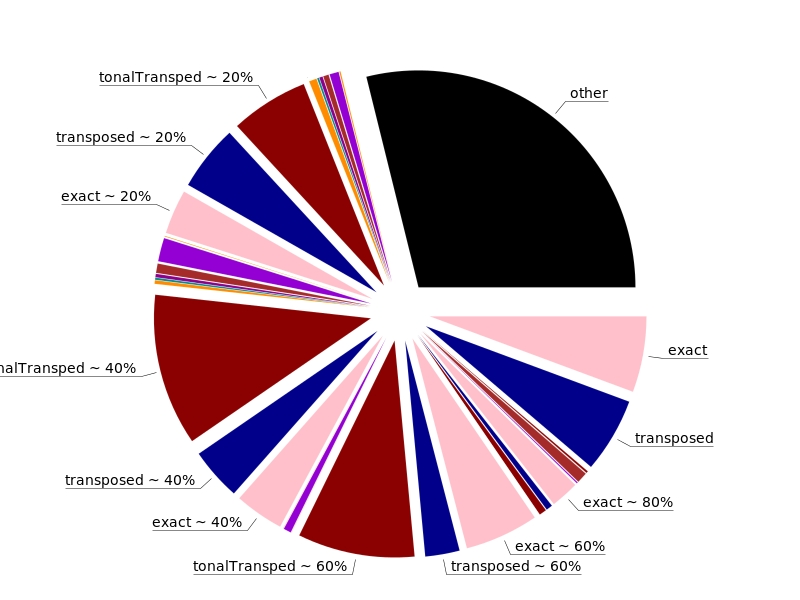
\includegraphics[width=.9\linewidth]{./img/ca.png}
\label{org69cb95a}
\end{center}
\end{column}

\begin{column}[T]{0.50\columnwidth}
\begin{center}
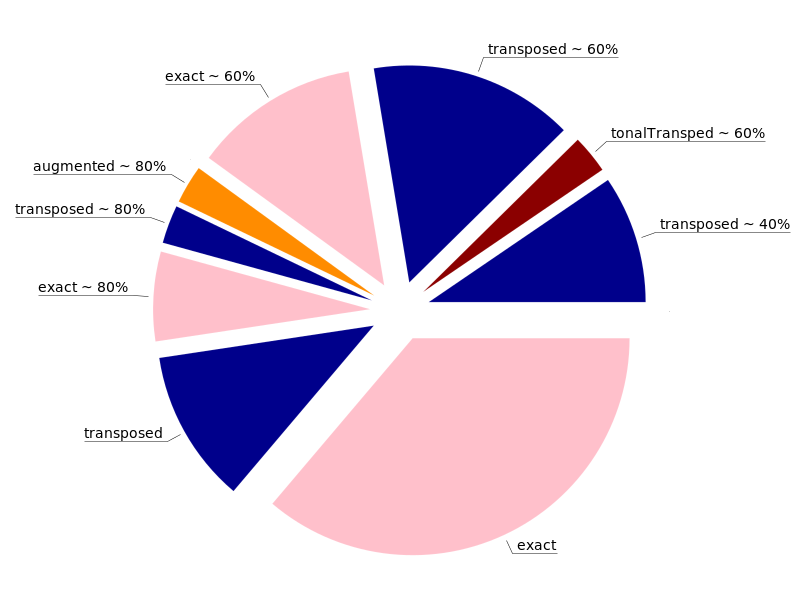
\includegraphics[width=.9\linewidth]{./img/ce.png}
\end{center}
\end{column}
\end{columns}
\end{block}

\begin{block}{Results: Folk}
Differences between human annotations and algorithmic results in a Dutch folk song dataset (MTC-ANN).
\begin{columns}
\begin{column}[T]{0.50\columnwidth}
\begin{center}
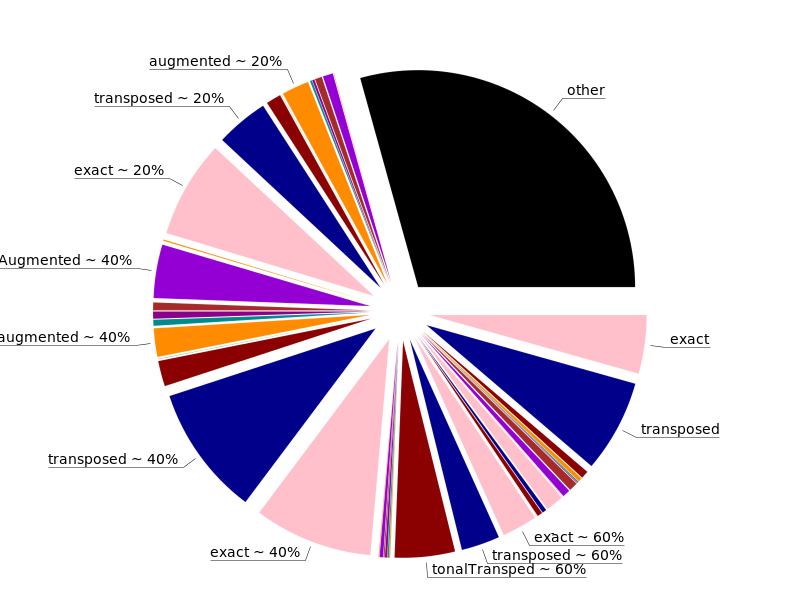
\includegraphics[width=.9\linewidth]{./img/fa.png}
\end{center}
\end{column}

\begin{column}[T]{0.50\columnwidth}
\begin{center}
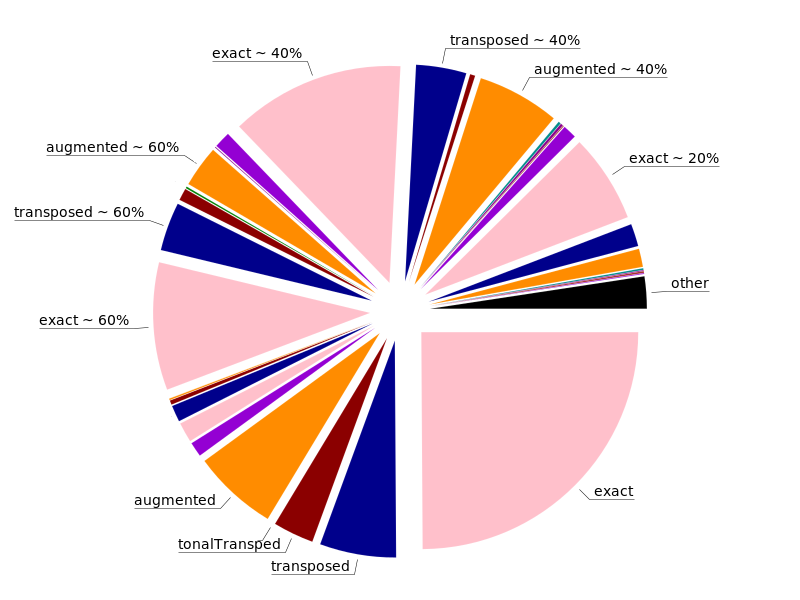
\includegraphics[width=.9\linewidth]{./img/fe.png}
\end{center}
\end{column}
\end{columns}
\end{block}
\begin{block}{Query and Discovery}
Querying comes for free!

\begin{columns}
\begin{column}[T]{0.80\columnwidth}
\small
\begin{minted}[linenos=false,bgcolor=white,breaklines=true]{haskell}
data UserQuery a = ToPattern a => Check Pattern :@ a
query1 :: UserQuery (Music Pitch)
query1 = (transpositionOf ~~ 0.5) :@ (line $ map ($qn) [c 4, e 4, g 4, c 5])
query2 :: UserQuery (Time, Time)
query2 = (transpositionOf ~~ 0.5) :@ (21 `upTo` 28)
\end{minted}
\end{column}
\end{columns}
\end{block}

\begin{block}{Conclusions}
\begin{itemize}
\item Category theory and Haskell in modelling and implementing higher order comparison: compare occurrence relations using musical transformations.
\item Implications for music: 
\begin{itemize}
\item Differences between musical pattern discovery algorithms and experts annotations.
\item Differences between different corpora.
\end{itemize}
\item Useful pattern query/discovery tool: \url{https://github.com/omelkonian/hs-pattrans}
\end{itemize}
\end{block}
\end{column}
\end{columns}
\end{frame}
\end{document}